\documentclass[12pt,a4paper]{article}
\usepackage{polski}
\usepackage[polish]{babel}
\usepackage{bbm}
\usepackage{bm}
\usepackage[T1]{fontenc}
\usepackage[utf8]{inputenc}
\usepackage[top=2cm, bottom=2cm, left=3cm, right=3cm]{geometry}
\usepackage{url}
\usepackage{graphics}
%\usepackage{graphicx}
\usepackage[pdftex]{graphicx}
\usepackage{float}
\usepackage{amsmath,amsthm}
\usepackage{enumitem}
\usepackage{epstopdf}
%\usepackage{indentfirst}
\usepackage[labelsep=period]{caption}

 
\setlist{nolistsep}


\AtBeginDocument{% Fragment zmieniający nazwy 'Rysunek' na 'Wykres' i 'Tablica' na 'Tabela'
        \renewcommand{\tablename}{Tabela}
        \renewcommand{\figurename}{Schemat}
}

\makeatletter
\newcommand{\linia}{\rule{\linewidth}{0.4mm}}


\floatstyle{plain}
\newfloat{image}{h!}{lop}
\floatname{image}{Rysunek}



\let \savenumberline \numberline
\def \numberline#1{\savenumberline{#1.}}


\renewcommand*{\@seccntformat}[1]{%
	  \csname the#1\endcsname
		    .\quad
}


\renewcommand{\maketitle}{\begin{titlepage}
		\vspace*{1cm}
    \begin{center}\small
    	Uniwersytet Wrocławski\\
    	Wydział Matematyki i Informatyki\\
    \end{center}
    \vspace{3cm}
    \noindent
    \linia
    \begin{center}
    	\LARGE{\textsc{\@title}}
         \end{center}
     \linia
    \begin{center}
    	\Large{Opis modułów}
         \end{center}
    \vspace{0.5cm}

    \begin{flushright}

    \begin{minipage}{5.5cm}

    	\small Autorzy:

    \normalsize {\@author} \par
    

    \end{minipage}
    \vspace{5cm}

     

     \end{flushright}

    \vspace*{\stretch{6}}

    \begin{center}

    \@date\\

    \end{center}

  \end{titlepage}%

}


\makeatother

\author{Jakub Stępniewicz (\textbf{233217})\\Rafał Maćkowski (\textbf{233170})\\Grupa {\bf I}}

\title{Symulator tramwaju\\ \small{Też możesz być motorniczym}}


\begin{document}
\maketitle
\tableofcontents
\vspace{5cm}
%	\begin{thebibliography}{9}
%	\bibitem{US} tz, W. Hill {\it Us}, Warszawa 2009.
%	\bibitem{MPK} \url{http://www.mpk.wroc.pl/}
%	\bibitem{SK} \url{http://www.skoda.cz/en/products/tramcars/tramcar-19-t/}
%	\bibitem{UE} \url{http://www.unrealengine.com/}
%	\bibitem{GO} \url{http://www.google.pl/#sclient=psy-ab&hl=pl&source=hp&q=%22symulator+tramwaju+skoda+16t%22&pbx=1&oq=%22symulator+tramwaju+skoda+16t}
%	\end{thebibliography}
\newpage
% 		Ok, najtrudniejsze za nami.		%
% 

\section{Wstęp}
Niniejszy dokument zawiera opis działania modułów symulatora, ich wzajemnych relacji oraz powiązania z elementami fizycznymi i interfejsami. 

\subsection{Schemat ogólny}
Właściwy symulator składa się z następujących modułów:
\begin{itemize}
\item {\bf Jednostka centralna} - komputer klasy PC odpowiedzialny za wykonywanie programów symulatora,
	jest także odpowiedzialny za przygotowanie wyświetlanego obrazu (wysyłanego potem do {\it
	systemu wyświetlania}), synchronizację danych pochodzących od {\it sterownika kokpitu} oraz
	współpracę z interfejsem instruktora.
\item {\bf Interfejs instruktora} - dostęp do interfejsu instruktora jest realizowany przez {\it jednostkę
	centralną}, przy pomocy podłączonych do niej urządzeń peryferyjnych. Umożliwia on kontrolę nad
	zewnętrznymi warunkami symulacji np. pogodą, natężeniem ruchu drogowego, czy losowymi sytuacjami na
	drodze.
\item {\bf Kontroler kokpitu} - oparty na mikrokontrolerze {\it ATMega128} system wbudowany
	kontrolujący stan wszystkich urządzeń znajdujących się w kokpicie.
\item {\bf System wyświetlania} - składa się z trzech {\it rzutników multimedialnych}, które
	wyświetlają obraz na ekranach zamontowanych w kokpicie. Dzięki integracji z systemem
	rozpoznawania położenia twarzy, wyświetlany obraz sprawia wrażenie trójwymiarowości.
\end{itemize}

Jednostka centralna komunikuje się z kontrolerem kokpitu oraz interfejsem instruktora za pomocą
specjalnie przystosowanych protokołów. Zbiera dane niezbędne do określenia aktualnych warunków
symulacji a następnie wyświetla aktualny stan tramwaju poprzez {\it wielofunkcyjny wyświetlacz}
zamontowany w kokpicie oraz system wyświetlania. Wzajemny przepływ danych między modułami został
zobrazowany na schemacie \ref{jeden}.
\begin{figure}[h]
	\begin{center}
		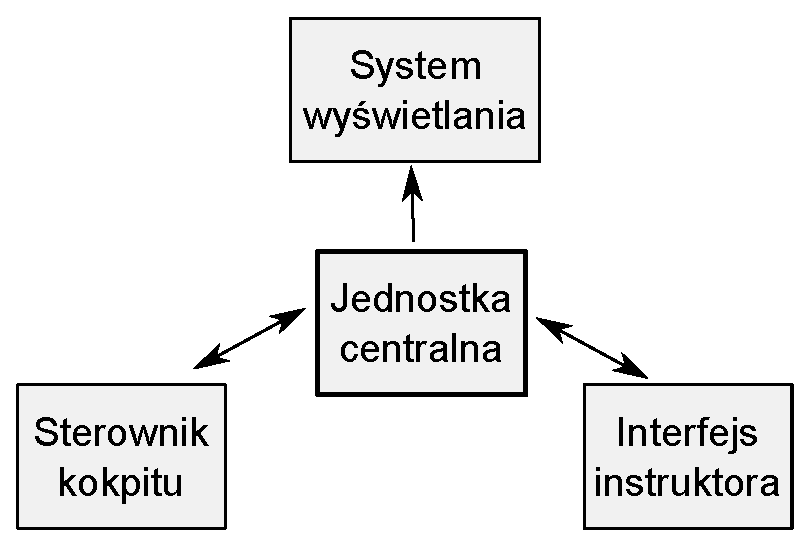
\includegraphics[scale=0.5]{img/jeden.eps}
		\caption{Ogólny schemat symulatora}
		\label{jeden}
	\end{center}
\end{figure}

\subsection{Sterownik kokpitu}
Sterownik kokpitu jest elementem odpowiedzialnym za komunikację pomiędy jednostką centralną a
motorniczym. Składa się on z licznych przycisków oraz wyświetlaczy, które umożliwiają monitorowanie
w czasie rzeczywistym wszystkich parametrów tramwaju. Schemat \ref{dwa} przedstawia podstawowe
elementy sterownika. 
\begin{figure}[h]
	\begin{center}
		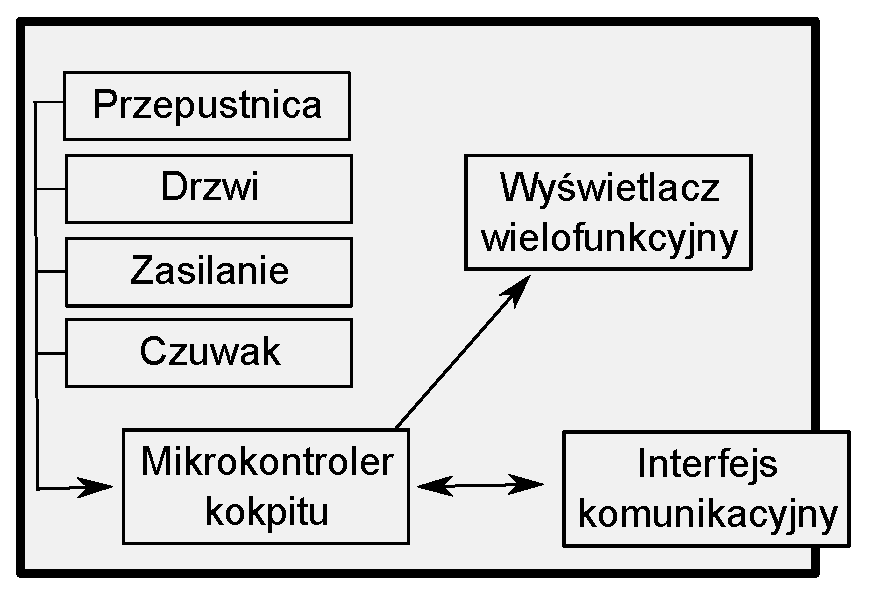
\includegraphics[scale=0.5]{img/dwa.eps}
		\caption{Sterownik kokpitu}
		\label{dwa}
	\end{center}
\end{figure}

Sygnały przesyłane przez przyciski, przełączniki i przepustnicę są przetwarzane wstępnie przez
mikrokontroler {\it ATMega128} a następnie przesyłane do jednostki centralnej, która podejmuje
decyzję o wpływie działań motorniczego na stan tramwaju. Odpowiedź jest przesyłana zarówno w postaci
informacji wyświetlanych na wyświetlaczu wielofunkcyjnym, jak i poprzez podświetlenie odpowiednich
przycisków czy przełączników.


\end{document}

